\section{Discussion and conclusions}
\label{sec:discussion}
We have four topics to discuss here:
\begin{itemize}
\item \textbf{Velocity map binning methods:} a technical discussion on the comparative merits of alternative MaNGA velocity map binning methods and IFU sizes to obtain best resolution Radon profile traces.
\item \textbf{The relationship between Radon profiles classes and morphology:} we discuss a possible correlation between Radon transform trace profile Types and galaxy morphology.
\item \textbf{Findings and conclusions:} a review of the significant findings of the project and presentation of our conclusions.
\item \textbf{Future work:} we present suggested topics for future work noted during the course of the project. 
\end{itemize}

\subsection{Velocity map binning methods}
\label{sec:binning-methods}
The MaNGA DAP utilises various spaxel binning models to process the IFU fibre bundle data into the output maps. The available binning schemes used to produce gas and stellar velocity maps, together with a brief description of each are listed below.

\begin{itemize}
    \item SPX - single spaxel measurements i.e. no binning.
    \item VOR10 - Voronoi binning, an adaptive spatial binning method where low signal-to-noise (S/N) ratio spaxels are grouped to achieve an overall S/N of 10  \citep{2003MNRAS.342..345C, 2019arXiv190100856W}.
    \item HYB10 - Hybrid binning: Voronoi S/N 10 binning for stellar velocity maps, but unbinned for emission line properties which are used to generate gas velocity maps.
\end{itemize}  

In this study we have utilised MaNGA datacubes released in DR15 MPL-7 which have been processed in the DAP using the hybrid HYB10 binning model, i.e. using VOR10 binning for the stellar velocity maps. However, the MaNGA project team currently have an internal dataset available, MPL-8. Datacubes in MPL-8 include VOR10 and SPX binning schema. We were interested to make a comparison of the Radon trace profiles generated from the datacubes using the Voronoi and SPX binning schemas. A limited sample of MPL-8 cubes were made available for this comparison exercise. We selected 2 galaxies from our samples with stellar velocity maps having poor spatial definition, and another 2 with good resolution in order to compare the Radon transform profiles using the Voronoi binning and SPX (unbinned) methods. The selected datacubes were firstly, examples of good resolution/definition in stellar velocity maps:

\begin{itemize}
    \item 7977-12704
    \item 8322-1901
\end{itemize}

and secondly, examples of poor resolution/definition in stellar velocity maps, i.e. having a blotchy appearance, due to spatial binning of low S/N spaxels, or with masked spaxels:

\begin{itemize}
    \item 9088-12703
    \item 8993-6104
\end{itemize}

The stellar velocity maps together with their Radon transform and trace profiles for these well defined example 7977-12704 are shown in Figure \ref{fig:binning-comparison}. The differences being the binning models of the input stellar velocity maps: Voronoi binning in the left-hand panel and SPX binning on the right. A comparison shows that there is little difference in the Radon transform and Radon profile plots. It is also apparent that the Radon transform algorithm for the SPX velocity maps yields a greater number of valid data points in the trace plot. We conclude that both VOR10 and SPX binned maps would lead to the same Type classification in these cases. This conclusion was also obtained for other galaxy showing good resolution in the stellar velocity map,  8322-1901 (figure not included). 

However, the same conclusion does not apply for the low resolution stellar velocity map examples, 8993-6104 shown in Figure \ref{fig:binning-comparison2} and 9088-12703 (figure not included). In these cases, at first sight, there are marked differences in the extent of spatial coverage and shapes of the velocity field PA, the Radon transform minimum and the Radon profile. In particular the control galaxy 8993-6104 displays a clearly asymmetric Radon profile with VOR10 binning, but could possibly be interpreted as an outer bend in the Radon profile trace of the SPX map. However, on closer inspection, looking at the  range the trace plots, the same bend feature at Radon transform coordinates [$\rho$, $\theta$]=[-6,+2],[20, 50] is apparent in both binning model plots. The asymmetric feature at $\rho$ \textgreater\ +2 apparent in the left Voronoi binned trace is not evident in the SPX output shown in the right-hand panel. Although these differences can be expected due to the exclusion of low S/N low spaxels in the SPX maps, crucially this can easily lead to a different visual classification result between the transforms of Voronoi binned and SPX velocity field maps. 
\begin{figure*}
    \centering
    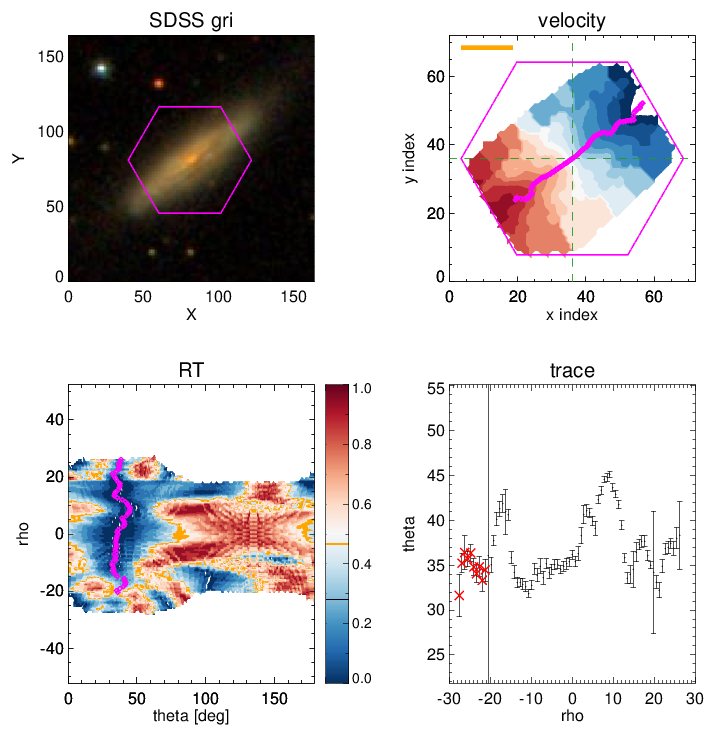
\includegraphics[width=\columnwidth]{images/RadonPlots/RT-SNIPS-NEW/7977-12704-VOR10-MILESHC-MILESHC-1-SNIP.png}
    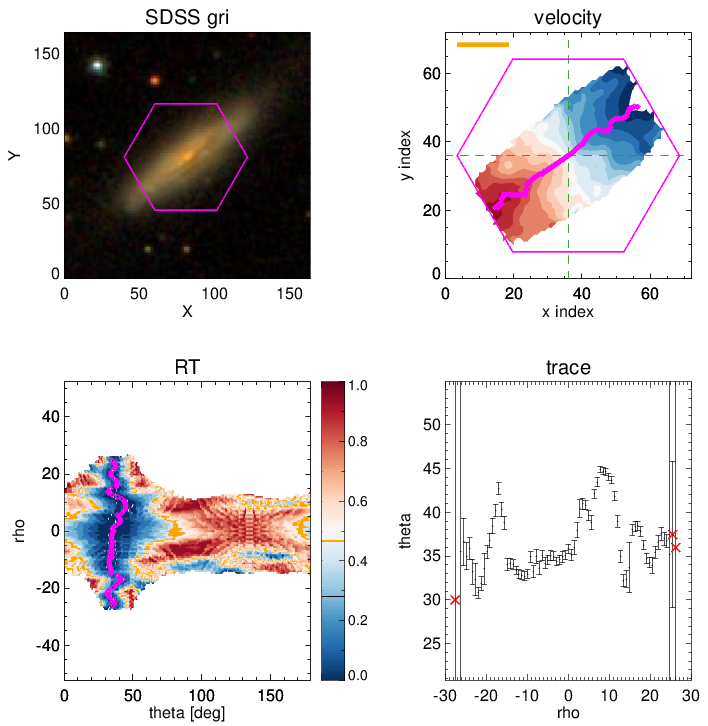
\includegraphics[width=\columnwidth]{images/RadonPlots/RT-SNIPS-NEW/7977-12704-SPX-MILESHC-MILESHC-1-SNIP.png}
    \caption[Comparison of velocity map binning schemes for a high resolution map]{Comparison of stellar velocity map binning methods using the Radon transform output graphic for the galaxy 7977-12704. The velocity map has good resolution using both schemes. In the left panel the transform RT and profile trace plots are generated from the stellar velocity map with Voronoi binning. The plots in the right panel were produced from the stellar velocity map using single spaxel SPX resolution. The layout of the 4 subplots in each panel is as described in Figure \ref{fig:8442-3704-complete}.}
    \label{fig:binning-comparison}
\end{figure*}

\begin{figure*}
    \centering
    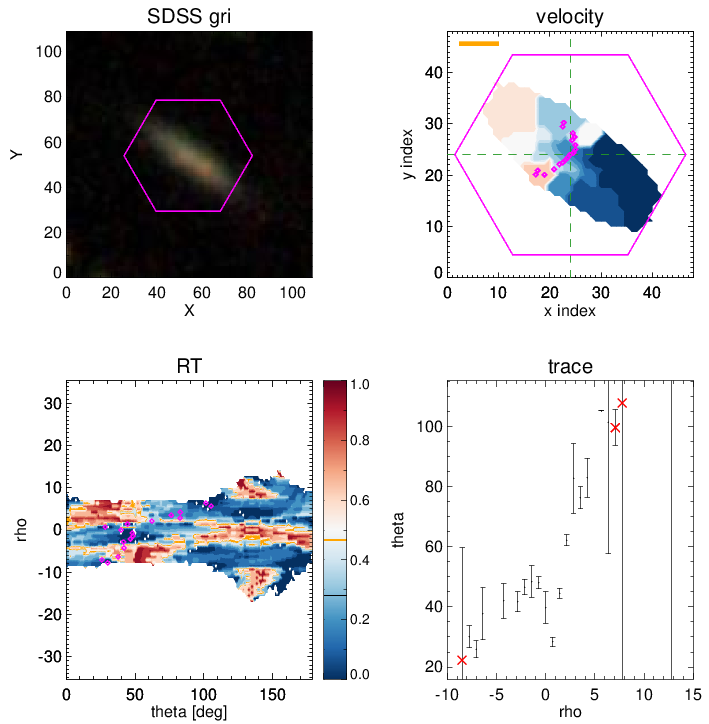
\includegraphics[width=\columnwidth]{images/RadonPlots/RT-SNIPS-NEW/8993-6104-VOR10-MILESHC-MILESHC-1-SNIP.png}
    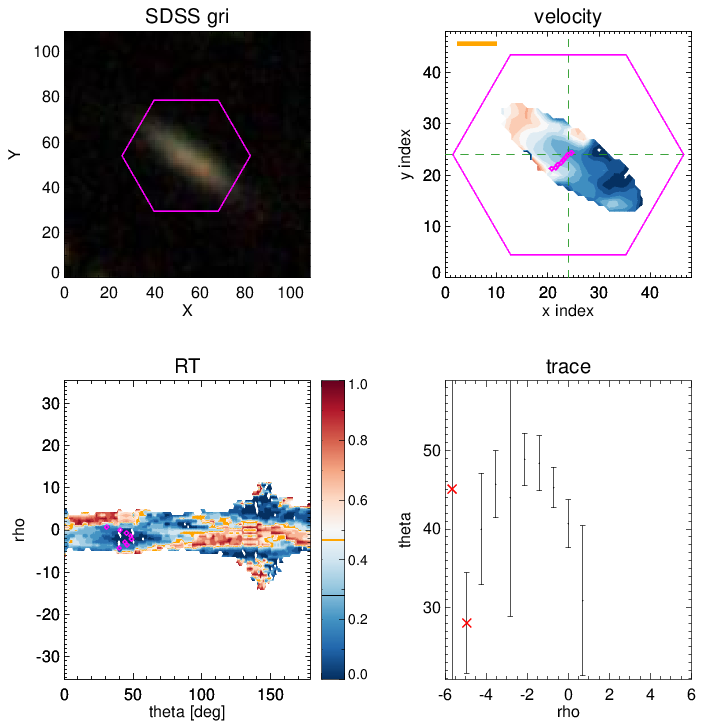
\includegraphics[width=\columnwidth]{images/RadonPlots/RT-SNIPS-NEW/8993-6104-SPX-MILESHC-MILESHC-1-SNIP.png}
    \caption[Comparison of velocity map binning schemes for a low resolution map]{Comparison of velocity map binning schemes for a low resolution map. Radon transform output graphic for the galaxy 8993-6104 with a low resolution stellar velocity map. In the left panel the transform RT and profile trace plots are generated from the stellar velocity map with Voronoi binning. The plots in the right panel were produced from the stellar velocity map using single spaxel SPX binning. The layout of the 4 subplots in each panel is as described in Figure \ref{fig:8442-3704-complete}.}
    \label{fig:binning-comparison2}
\end{figure*}




\subsection[Correlation between Radon profiles and morphology]{Correlation between Radon profile types and morphological features}
\label{correlations}
\cite{2018MNRAS.480.2217S} made a considerable effort to explore a possible correlation between the observed frequencies of the 5 Radon profile types (Type-C, Type-A, Type-IB, Type-OB and Type-OB+IB) and underlying morphological features determined from the Galaxy Zoo morphology classification project. They found some evidence of weak associations between Radon profile trace type and morphological features, as discussed in detail in their Section 5. These correlations are subjective and certainly not exclusive, and care must be taken to follow their arguments closely. The most prevalent of the identified relationships can be broadly interpreted as follows:
\begin{itemize}
    \item Type-C: Constant profile - frequently apparent in unbarred galaxies.
    \item Type-A: Asymmetric - can be associated with tidal interactions.
    \item Type-IB: Inner bends - prevalent in strongly barred galaxies.
    \item Type-OB: Outer bends - associated with kinematic warps.
\end{itemize}

\blue{Following this discussion the prevailing reasoning is that outer bend-type features, Type-OB, may be associated with kinematic warps and indicative of past mergers. Also Type-C (constant) profiles were expected to be associated with indicate uniform, undisturbed velocity fields. As reported in the results Section \ref{sec:comparison-of-results} we found that 5 out of 14 PSBs with large $\Delta$PA$_{k}$ offsets were assigned Radon profile trace classification of Type-OB. We emphasise, however, that this result was determined by Classifier A, and there is no consensus with either Classifier B or in the limited number of automatic classifications that were available for our galaxies. Setting this point aside there may be some correlation between Radon profile Type-OB, large $\Delta$PA$_{k}$ and past major mergers driving quenching in post-starburst galaxies.}

\subsection{Findings}
\label{findings}

%TC:ignore
\green{Include a bit linking high S\'ersic index (CPSBs), high DeltaPAs (CPSBs), the K-S test, spheroidal morphology and CPSBs. How do we do that?}
%TC:endignore

Generally CPSBs show a wide range of kinematic position angle differences $\Delta$PA$_{k}$ \textgreater 30\textdegree\ with many in the range 90 \textless\ $\Delta$PA$_{k}$ \textless\ 180\textdegree. RPSBs show a smaller range in $\Delta$PA$_{k}$ with only a few over 90\textdegree. The majority of control galaxies have small kinematic position angle differences, mainly less than 25\textdegree. Significant misalignment in the gas and stellar velocity fields of CPSBs, and to a lesser extent RPSBs, is indicative of past or ongoing disturbances as could be expected from major mergers.
We note that the distribution $\Delta$PA$_{k}$ is markedly different when comparing CPSBs with CPSB controls. This trait is also present, but to a lesser extent, in the comparison of the RPSB $\Delta$PA$_{k}$ with their controls. The distribution in differential kinematic position angles is similar for both control groups. These observations are supported by the results of K-S analysis in Section \ref{sec:K-S-test} where we find the difference in $\Delta$PA$_{k}$ of both PSB groups compared to their control groups to be statistically significant. \green{From this we conclude that there is evidence presented from the $\Delta$PA$_{k}$ distributions, the K-S statistical analysis performed on these $\Delta$PA$_{k}$ distributions, together with the distributions in S\'ersic index that there is a evolutionary sequence from the normal (control) galaxies, to the disc-like RPSBs and on to the redder spheroidal CPSBs. The quenching of star formation in ring-shaped features in RPSBs and the central regions of CPSBs provides compelling evidence of past major mergers, triggering morphological transformation from late-type galaxies to spheroids and an evolutionary transition from the blue cloud, through the green valley, and on towards the red sequence.}

We compared the Radon profile trace results obtained from stellar velocity maps employing Voronoi VOR10 binning versus the single spaxel SPX unbinned schema. We obtained cleaner trace profiles (i.e. easier to classify) with a greater number of valid data points and tighter error bars from high S/N maps based on single spaxel SPX binning. For future studies, given a large enough sample of PSBs, we should avoid Voronoi binned maps where possible and use SPX maps a cut of S/N \textgreater say 3-5 in single spaxels.

Kinematic PA analysis versus Radon transform: as described in Section \ref{sec:motivation} the Radon transform provides distinct advantages over the kinematic $\Delta$PA$_{k}$  method. Radon transforms provide a detailed trace of position angle across the velocity field enabling local regions of radial variation to be identified. Kinematic PAs require both stellar and gas velocity fields to be mapped but post-starburst galaxies may possess little gas. The Radon transform can trace disturbances as evidence of mergers using the stellar velocity field alone.

Kinematic warps in the stellar discs of early-type field galaxies can be attributed to multiple stellar components suggestive of past dry mergers \citep{2005AJ....130.2647V}, although warps can also be sustained by tidal interactions.
From this we draw the simple conclusion that Radon trace profiles displaying outer bends, Type-OB or Type-OB+IB can be considered prospective candidates past major mergers, or post-mergers. From Table \ref{tab:Radon-VC-results} we find that 10 of of 27 CPSBs (37\%) reveal Type-OB or Type-OB+IB Radon profile signatures. As an area for future study we should consider a similar exercise to utilise the Galaxy Zoo morphology classifications together with Radon profile feature types as identified in this present study. 

Visual classification of Radon profile types was found to be very difficult, our classifiers agreed on this point. In addition our classifiers arrived at varying interpretations of profile type class for most of the galaxies. Although the same written classification procedure was followed, the method was quite loosely defined, recognising the difficulties in relating the race plots to the examples. With so few classifiers involved we conclude that there is significant classification error present in our results, remembering the the Galaxy Zoo project engaged $\sim10^5$ classifiers to minimise classification error.

The results of the visual classification of the 5 Radon trace type profiles for CPSBs, RPSBs and their control groups as presented in Table \ref{tab:Radon-VC-results} and shown graphically in Figure \ref{fig:Radon-grouped-barchart} are quantitatively similar in number. This was unexpected and is presently not fully explained. We can, however, expect more galaxies with constant features in the RPSB groups than the CPSBs as RPSBs exhibit PSB features in local regions only while we can expect a higher percentage of the non-linear features, i.e. inner and outer bends and composite bend features Type-OB+IB, to be apparent in the trace profiles of CPSBs due to their central and more widespread post-starburst regions. Incorporating the the results from the second classifier a picture emerges that Type-OB features are 70\% more prevalent in both the CPSB sample to controls, and RPSBs to their controls. 

\subsection{Summary}
\label{summary}
In the past major mergers have been detected using imaging techniques. In this project we have attempted to identify past major mergers in PSB galaxies, firstly by investigating the distributions of differences in stellar and gas velocity field kinematic position angles, and secondly by using the Radon transform method to reveal radial variation in kinematic position angles. This has not proved conclusive. More work is required on the classification of kinematic features apparent in the Radon profile trace plots. However, \cite{2019DDA....5020304N} have recently announced work on a method which promises to increase the accuracy of merger detection using a method that integrates imaging and kinematic analysis techniques. This extended method will combine SDSS imaging (providing morphological observations) with MaNGA  kinematic maps, towards enhanced identification of merger and post-merger signatures. When available, this technique should be applied to our PSB and control samples to detect evidence of past mergers. With this technique we may be able to increase our likelihood estimates of positive detection of past major merger events in post-starburst galaxies.

